\documentclass[11pt,psfig]{article}
\usepackage{epsfig}
\usepackage{times}
\usepackage{amssymb}
\usepackage{float}

\newcount\refno\refno=1
\def\ref{\the\refno \global\advance\refno by 1}
\def\ux{\underline{x}}
\def\uw{\underline{w}}
\def\bw{\underline{w}}
\def\ut{\underline{\theta}}
\def\umu{\underline{\mu}} 
\def\bmu{\underline{\mu}} 
\def\be{p_e^*}
\newcount\eqnumber\eqnumber=1
\def\eq{\the \eqnumber \global\advance\eqnumber by 1}
\def\eqs{\eq}
\def\eqn{\eqno(\eq)}

 \pagestyle{empty}
\def\baselinestretch{1.1}
\topmargin1in \headsep0.3in
\topmargin0in \oddsidemargin0in \textwidth6.5in \textheight8.5in
\begin{document}
\setlength{\parskip}{1.2ex plus0.3ex minus 0.3ex}


\thispagestyle{empty} \pagestyle{myheadings} \markright{G}



\title{CS 266 Homework 8}
\author{Zachary DeStefano, PhD Student, 15247592}
\date{Due Date: June 5, 2014}

\maketitle

\vfill\eject

\section*{Problem 11.2}

We will always be going through each of the n points. \\
In the worst case, when we go through a point, almost every current facet except a constant number has to be deleted.\\
A new conflict graph is then made and for each face, \\
all the remaining points have to be checked to reconstruct the graph. \\
\\
Deleting the current facets will take O(n) time. \\
Making a new conflict graph will be O(n) time for each facet and there are up to O(n) facets, so for each point there could be O($n^2$) operations to reconstruct the conflict graph. \\
This has to be done for each point so in the worst case, the running time is $O(n^3)$. \\
\\
An example:\\
Let's say we have a tower-like structure, where there is a face at the bottom with $\frac{n}{2}$ points and then perpendicular to that face are $\frac{n}{2}$ points that are almost collinear above it. If we pick the bottom face first and then pick the points in ascending order by distance from the bottom, then at each point, we have to completely delete and rebuild the conflict graph and the hull as all but the bottom facet would be changed. This is a case that needs $\Theta(n^3)$ time. It is illustrated below. In the figure below, if the bottom triangle and 1 makes your starting tetrahedron, then you process point 2 and then point 3, the running time will be as bad as possible. 

\begin{figure}[H]
\centering
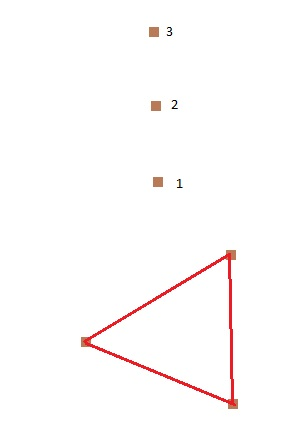
\includegraphics[height=2.5in]{hw8prob1diagram.jpg}
\caption{Bad Convex Hull points}
\end{figure}

\newpage

\section*{Problem 11.4}

In the proof of Lemma 11.6, the $n \cdot log(n)$ term is established because the summation uses the number of edges as $6r-12$. \\
In this case however, we can assume that the number of edges is $k \cdot r^{\alpha}$ for some constant $k$ \\
If we looking the following summation from that proof:
\[
\sum_{e} card(P(e)) \leq \sum_{r=1}^n 16 \frac{n-r}{r} \frac{6r-12}{r}
\]
We can now replace it with the following
\[
\sum_{e} card(P(e)) \leq \sum_{r=1}^n k \frac{n-r}{r} \frac{r^{\alpha}}{r}
\]
For simplicity, we know that $n-r \leq n$ and we will let $\beta=2-\alpha$. We can now say that
\[
\sum_{e} card(P(e)) \leq \sum_{r=1}^n k \frac{n}{r^{\beta}}
\]
\[
\sum_{e} card(P(e)) \leq k \cdot n (\sum_{r=1}^n \frac{1}{r^{\beta}})
\]
Since $\beta$ is greater than 1, the series would converge to a constant value. Thus we can further say that
\[
\sum_{e} card(P(e)) \leq k \cdot n
\] 
Thus our running time is $O(n)$

\newpage

\section*{Problem 11.8}

Describe a randomized incremental algorithm to compute the intersection
of half-planes, and analyze its expected running time. Your algorithm
should maintain the intersection of the current set of half-planes.
To figure out where to insert a new half-plane, maintain a conflict graph
between the vertices of the current intersection and the half-planes that
are still to be inserted.\\
\\
The intersection will be described by a set of vertices in a specific order making up the intersection as well as indicators of which side of the border the intersection lies on. \\
For each vertex, we will maintain a pointer to the half-planes that it is inside of. This will be the conflict graph. \\
There will be vertices representing lines going to infinity.\\
There will be 4 additional vertices representing the 4 infinite corners\\
\\
When a new line is picked randomly, we see which vertices intersect its half-plane. We include only those vertices and add two new vertices for the new points. \\
\\
Here is the algorithm:\\
Pick two lines randomly and compute their intersection. The intersection now consists of 3 vertices. \\
For each vertex in the intersection, connect them to the lines whose half-planes they are inside. \\
For each remaining line L in random order:\\
- If no vertex is in L's half-plane return empty intersection\\
- Else If all vertices are in L's half-plane, then continue to next line\\
- Else \\
- - Delete the vertices from the graph that are not in L's half-plane\\
- - Find edges $e_1$ and $e_2$ whose vertices were consecutive in the intersection but where one vertex was in L's half-plane and one was not\\
- - Construct new vertices $v_1$ and $v_2$ which are the intersection of $e_1$ and $e_2$ with L. \\
- - Add $v_1$ and $v_2$ to the intersection and compute which of the remaining half-planes they are inside. \\
\\
Worst Running time:\\
It will be going through $n$ lines. \\
For each line, it could go through at most $n$ vertices or lines in each of the steps. \\
For each vertex or line, there are a constant number of operations being done. \\
Thus in the worst case, the running time is $O(n^2)$. \\
\\
Expected Running time:\\
We will assume that there is not an empty intersection. \\
The question then is we will continue or do we have to recompute the intersection. \\
The expected running time is thus $\sum_{i=1}^n n \cdot Pr(I \notin L)$\\
We will assume the probability reflects the fact that we have 1 line to find and $i$ lines computed, so at each step it is $\frac{1}{i}$. \\
This gives us 
\[
T(n) = n \sum_{i=1}^n \frac{1}{i} \leq n \cdot log(n)
\]

\end{document}








